%%%%%%%%%%%%%%%%%%%%%%%%%%%%%%%%%%%%%%START PREAMBLE THAT IS THE SAME FOR ALL EXAMPLES
\documentclass{article}

\usepackage{Sweave}
\usepackage{graphicx}
\usepackage{tabularx}
\usepackage{hyperref}
\usepackage{natbib}
\usepackage{pdflscape}
\usepackage{array}
\usepackage{gensymb}
\usepackage{amsmath}

\usepackage{xr}

%\usepackage[backend=bibtex]{biblatex}
%Strongly recommended
%put your figures in one place
%\SweaveOpts{prefix.string=figures/, eps=FALSE} 
%you'll want these for pretty captioning
\usepackage[small]{caption}

\setkeys{Gin}{width=0.8\textwidth}  %make the figs 50 perc textwidth
\setlength{\captionmargin}{30pt}
\setlength{\abovecaptionskip}{10pt}
\setlength{\belowcaptionskip}{10pt}
% manual for caption  http://www.dd.chalmers.se/latex/Docs/PDF/caption.pdf
\topmargin -1.5cm        
\oddsidemargin -0.04cm   
\evensidemargin -0.04cm  % same as oddsidemargin but for left-hand pages
\textwidth 16.59cm
\textheight 21.94cm 

\pagestyle{empty}       
% Uncomment if don't want page numbers
\parskip 7.2pt           % sets spacing between paragraphs
%\renewcommand{\baselinestretch}{1.5} 	% Uncomment for 1.5 spacing between lines
\parindent 0pt% sets leading space for paragraphs
\usepackage{setspace}
%\doublespacing

%%%%%%%%%%%%%%%%%%%%%%%%%%%%%%%%%%%%%%END PREAMBLE

%Start of the document
\begin{document}

%\SweaveOpts{concordance=TRUE}

\bibliographystyle{../refs/bibstyles/amnat.bst}

\title{Supplemental methods for Shifting phenology of an endangered apex predator tracks changes in its favored prey}
\date{\today}
\maketitle
\author{A.K. Ettinger, C. Harvey, J. Samhouri, B. Hanson, C. Emmons, J. Olson, E. Ward}
%%%%%%%%%%%%%%%%%%%%%%%%%%%%%%%%%%%%%%%%%%%%%%%%%%%

\section* {Effects of changes in effort on estimated phenological change (simulations)}
To better understand how increased effort across the time-series (i.e., increased numbers of sightings over time) may affect estimates of trends in phenology, we simulated data sets of whale presence during two seasons equivalent to those in our data set (spring/summer, which was 1 May through 31 Sept, or 153 days, and fall/winter, which was 1 October through 1 Feb, or 123 days). We used whale presence probabilities of 0.85 for the Central Salish Sea and 0.6 for Puget Sound (the means in our data set for each region, from 1978-2017) and kept them constant over 40 simulated years. We then created an observation data set, in which effort (the number of observations) varied. During the low effort time period (years 1-20), the number of observations had a mean of 15 per year for Puget Sound and 104 per year in the Central Salish Sea (matching the means for these regions from 1978-1997 in the OrcaMaster database). During the high effort time period (years 21-40 in our simulated data set), the number of annual observations had a mean of 39 for Puget Sound and 133 for the Central Salish Sea (matching those in the OrcaMaster database from 1998-2017). We then calculated first- and last- observations dates for each simulated year. We ran these simulations 100 times and calculated the difference between the low effort and high effort time periods. We compared these to the mean differences in first- and last-observation dates across time periods in the OrcaMaster database, for each region, to understand whether observed changes may be due to changes in effort over time, rather than changes in killer whale activity. 

\par Estimted change across the full time series = 
\par Estimted shift in recent time period along = 
\par The large increase in effort has likely affected trends, especially across the full time series.  However, the expected change due to increased effort opposes the patterns we observed in recent years for the Central Salish Sea (i.e., we would expect earlier arrival, later departure, and increased occurrence probability;  see Supplemental Materials for details, especially Fig. SX). 

\par Changing the breakpoint to 2007 or 2008 did not qualitatively alter results (Fig. SX)

\section* {Supplemental Tables}
\par Table 1: Salmon runs included in puget sound and central salish sea analyses 
\par Table of trends in different phenophases for salmon (or perhaps combine with above table?)
\par Pod-specific shifts at lime kiln

% latex table generated in R 3.6.0 by xtable 1.8-4 package
% Mon Dec 16 14:03:49 2019
\begin{table}[ht]
\centering
\caption{\textbf{Estimated linear trends in peak-, start-of-, and end-of-season SRKW phenology} in Puget Sound proper and the central Salish Sea, from occupancy model estimates of presence probabilites. `Peak' is the day of year with the maximum probability of presence (or the mean across day of year, if there are multiple days with the peak probability of presence). To estimate the start of the season, we identified the earliest day of year with an estimated presence probility greater than 0.5. To estimate the end of the season, we identified the latest day of year with an estimated presence probility greater than 0.5. 50 percent credible intervals are in parantheses.} 
\label{tab:modsz}
\begingroup\footnotesize
\begin{tabular}{|p{0.04\textwidth}|p{0.20\textwidth}|p{0.1\textwidth}|p{0.08\textwidth}|p{0.05\textwidth}|p{0.05\textwidth}|p{0.05\textwidth}|p{0.05\textwidth}|p{0.05\textwidth}|p{0.05\textwidth}|}
  \hline
Pod & Region & Season & Phase & mean & 25\% & slope.uci & mean & 25\% & 75\% \\ 
  \hline
J & Puget Sound & Fall & peak & 1.14 & 0.87 & 1.41 & 0.74 & -0.42 & 1.86 \\ 
  J & Puget Sound & Fall & first & 0.54 & 0.08 & 0.99 & 2.67 & 1.60 & 3.77 \\ 
  J & Puget Sound & Fall & last & 0.97 & 0.52 & 1.40 & -0.95 & -1.91 & -0.03 \\ 
  J & Central Salish Sea & Summer & peak & 1.13 & 0.74 & 1.53 & 5.16 & 2.14 & 8.47 \\ 
  J & Central Salish Sea & Summer & first & -0.75 & -0.90 & -0.61 & 1.11 & 0.94 & 1.20 \\ 
  J & Central Salish Sea & Summer & last & 1.12 & 0.95 & 1.27 & 0.47 & 0.29 & 0.65 \\ 
  K & Puget Sound & Fall & peak & 1.77 & 1.48 & 2.07 & 1.92 & 0.67 & 3.08 \\ 
  K & Puget Sound & Fall & first & 1.67 & 1.14 & 2.23 & 2.27 & 1.01 & 3.62 \\ 
  K & Puget Sound & Fall & last & 2.75 & 2.20 & 3.32 & 1.50 & 0.89 & 2.11 \\ 
  K & Central Salish Sea & Summer & peak & 0.90 & 0.60 & 1.20 & 1.14 & 0.26 & 2.04 \\ 
  K & Central Salish Sea & Summer & first & -0.36 & -0.62 & -0.10 & 0.83 & 0.30 & 1.60 \\ 
  K & Central Salish Sea & Summer & last & 0.69 & 0.46 & 0.89 & -0.79 & -1.44 & -0.20 \\ 
   \hline
L & Puget Sound & Fall & peak & 1.07 & 0.87 & 1.28 & -0.46 & -1.00 & -0.01 \\ 
  L & Puget Sound & Fall & first & 1.68 & 1.04 & 2.36 & 1.46 & 0.25 & 2.66 \\ 
  L & Puget Sound & Fall & last & 1.04 & 0.36 & 1.76 & -1.70 & -2.27 & -1.13 \\ 
   \hline
L & Puget Sound & Fall & peak & 1.06 & 0.64 & 1.46 & -0.39 & -1.36 & 0.66 \\ 
  L & Puget Sound & Fall & first & 1.74 & 0.46 & 2.93 & 1.46 & -0.92 & 3.79 \\ 
  L & Puget Sound & Fall & last & 1.02 & -0.38 & 2.34 & -1.33 & -2.59 & 0.02 \\ 
   \hline
L & Central Salish Sea & Summer & peak & 0.21 & -0.05 & 0.47 & -1.00 & -1.96 & -0.01 \\ 
  L & Central Salish Sea & Summer & first & -1.80 & -2.09 & -1.52 & 0.54 & 0.23 & 0.87 \\ 
  L & Central Salish Sea & Summer & last & 1.04 & 0.80 & 1.27 & -0.20 & -0.41 & 0.03 \\ 
   \hline
L & Central Salish Sea & Summer & peak & 0.22 & -0.29 & 0.73 & -1.08 & -2.93 & 0.77 \\ 
  L & Central Salish Sea & Summer & first & -1.80 & -2.34 & -1.25 & 0.64 & -0.05 & 1.31 \\ 
  L & Central Salish Sea & Summer & last & 1.08 & 0.66 & 1.52 & -0.19 & -0.61 & 0.20 \\ 
   \hline
\end{tabular}
\endgroup
\end{table}
\par Table comparing estimates of shifts
% latex table generated in R 3.6.0 by xtable 1.8-4 package
% Mon Dec 16 14:03:49 2019
\begin{table}[ht]
\centering
\caption{\textbf{Estimated linear trends in peak-, start-of-, and end-of-season SRKW phenology} in Puget Sound proper and the central Salish Sea, from occupancy model estimates of presence probabilites. `Peak' is the day of year with the maximum probability of presence (or the mean across day of year, if there are multiple days with the peak probability of presence). To estimate the start of the season, we identified the earliest day of year with an estimated presence probility greater than 0.5. To estimate the end of the season, we identified the latest day of year with an estimated presence probility greater than 0.5. 50 percent credible intervals are in parantheses.} 
\label{tab:modsz}
\begingroup\footnotesize
\begin{tabular}{|p{0.04\textwidth}|p{0.20\textwidth}|p{0.1\textwidth}|p{0.08\textwidth}|p{0.20\textwidth}|p{0.20\textwidth}|}
  \hline
Pod & Region & Season & Phase & 1978-2017 trend & 2002-2017 trend \\ 
  \hline
J & Puget Sound & Fall & peak & 1.14 (0.87 - 1.41) & 0.74 (-0.42 - 1.86) \\ 
  J & Puget Sound & Fall & first & 0.54 (0.08 - 0.99) & 2.67 (1.6 - 3.77) \\ 
  J & Puget Sound & Fall & last & 0.97 (0.52 - 1.4) & -0.95 (-1.91 - -0.03) \\ 
  J & Central Salish Sea & Summer & peak & 1.13 (0.74 - 1.53) & 5.16 (2.14 - 8.47) \\ 
  J & Central Salish Sea & Summer & first & -0.75 (-0.9 - -0.61) & 1.11 (0.94 - 1.2) \\ 
  J & Central Salish Sea & Summer & last & 1.12 (0.95 - 1.27) & 0.47 (0.29 - 0.65) \\ 
  J & Puget Sound & Full Year & peak & 2.17 (0.95 - 3.39) & 1.59 (-4.2 - 8.59) \\ 
  J & Puget Sound & Full Year & first & 1.9 (-0.42 - 4.29) & -3.57 (-10.1 - 2.91) \\ 
  J & Puget Sound & Full Year & last & 1.24 (-0.54 - 3.14) & -3.7 (-7.39 - 0.43) \\ 
  J & Central Salish Sea & Full Year & peak & -0.05 (-1.57 - 1.42) & 3.36 (-3.75 - 9.64) \\ 
  J & Central Salish Sea & Full Year & first & -2.22 (-2.94 - -1.52) & -1.8 (-2.68 - -0.95) \\ 
  J & Central Salish Sea & Full Year & last & 2.22 (1.67 - 2.75) & 2.19 (1.18 - 3.19) \\ 
   \hline
K & Puget Sound & Fall & peak & 1.77 (1.48 - 2.07) & 1.92 (0.67 - 3.08) \\ 
  K & Puget Sound & Fall & first & 1.67 (1.14 - 2.23) & 2.27 (1.01 - 3.62) \\ 
  K & Puget Sound & Fall & last & 2.75 (2.2 - 3.32) & 1.5 (0.89 - 2.11) \\ 
   \hline
K & Central Salish Sea & Summer & peak & 0.9 (0.6 - 1.2) & 1.14 (0.26 - 2.04) \\ 
  K & Central Salish Sea & Summer & first & -0.36 (-0.62 - -0.1) & 0.83 (0.3 - 1.6) \\ 
  K & Central Salish Sea & Summer & last & 0.69 (0.46 - 0.89) & -0.79 (-1.44 - -0.2) \\ 
   \hline
K & Puget Sound & Full Year & peak & 3.74 (2.72 - 4.62) & 3.76 (-1.4 - 11.37) \\ 
  K & Puget Sound & Full Year & first & 2.33 (0.11 - 4.41) & 14.67 (8.77 - 20.14) \\ 
  K & Puget Sound & Full Year & last & 3.91 (2.35 - 5.49) & 5.87 (1.07 - 11.9) \\ 
   \hline
K & Central Salish Sea & Full Year & peak & 1.53 (0.66 - 2.45) & 5.12 (2.08 - 7.6) \\ 
  K & Central Salish Sea & Full Year & first & -2.35 (-3.24 - -1.38) & -2.27 (-6.29 - 1.9) \\ 
  K & Central Salish Sea & Full Year & last & 2.59 (1.85 - 3.35) & 1.7 (0.27 - 3.08) \\ 
   \hline
L & Puget Sound & Fall & peak & 1.07 (0.87 - 1.28) & -0.46 (-1 - -0.01) \\ 
  L & Puget Sound & Fall & first & 1.68 (1.04 - 2.36) & 1.46 (0.25 - 2.66) \\ 
  L & Puget Sound & Fall & last & 1.04 (0.36 - 1.76) & -1.7 (-2.27 - -1.13) \\ 
  L & Puget Sound & Fall & peak & 1.06 (0.64 - 1.46) & -0.39 (-1.36 - 0.66) \\ 
  L & Puget Sound & Fall & first & 1.74 (0.46 - 2.93) & 1.46 (-0.92 - 3.79) \\ 
  L & Puget Sound & Fall & last & 1.02 (-0.38 - 2.34) & -1.33 (-2.59 - 0.02) \\ 
  L & Central Salish Sea & Summer & peak & 0.21 (-0.05 - 0.47) & -1 (-1.96 - -0.01) \\ 
  L & Central Salish Sea & Summer & first & -1.8 (-2.09 - -1.52) & 0.54 (0.23 - 0.87) \\ 
  L & Central Salish Sea & Summer & last & 1.04 (0.8 - 1.27) & -0.2 (-0.41 - 0.03) \\ 
  L & Central Salish Sea & Summer & peak & 0.22 (-0.29 - 0.73) & -1.08 (-2.93 - 0.77) \\ 
  L & Central Salish Sea & Summer & first & -1.8 (-2.34 - -1.25) & 0.64 (-0.05 - 1.31) \\ 
  L & Central Salish Sea & Summer & last & 1.08 (0.66 - 1.52) & -0.19 (-0.61 - 0.2) \\ 
  \end{tabular}
\endgroup
\end{table}


\section* {Supplemental Figures}
\par Time series of peak prob. occurence for K and L pods
\par Time series for first- and last- dates when occurrence probabilty is greater than 0.5 for J,K,L pods
\par raw data summaries: caption The shift toward later arrival in the central Salish Sea is evident in the number of whale days, averaged across the most recent portion of the time series (2009-2017) compared to the average of the earlier half of the timeseries we analyzed  A,B).  Shading around lines represents standard deviation for left panels, Gray shading in left panels shows the time year during which regional models were fit.


\par Figure with Changing the breakpoint of 2006 in Figure 3to 2007 or 2008 did not qualitatively alter results (Fig. SX)
Coincident with these phenological trends, the number of whale days has also changed across the time-series (Fig. SX). Since 2001, the number of whale days has decreased in the Central Salish Sea, across all pods, whereas in Puget Sound proper the number of whale days did not show a consistent trend (Fig. SX). From 1978 to 2017, the number of whale days increased in both regions (and for all pods). 
\par To Do 
Add to supplemental Materials: 
(a) Table S1. Details on salmon runs used to quantify phenology (annual run size, species, source)
(b) Table S2. comparing estimates of shifts 
(b) Figure S1. Time series of peak prob. occurrence for K and L pods 
(c) Time series for first- and last- dates when occurrence probability is greater than 0.5 for J,K,L pods 
(d) show relationship between lime kiln, and central salish sea phenology
(e) model stats- demonstrate that the models work/make sense 
(f) Expected phenological change due to change in effort alone (simulations)- do this for the recent time span as well?

\begin{figure}[p]
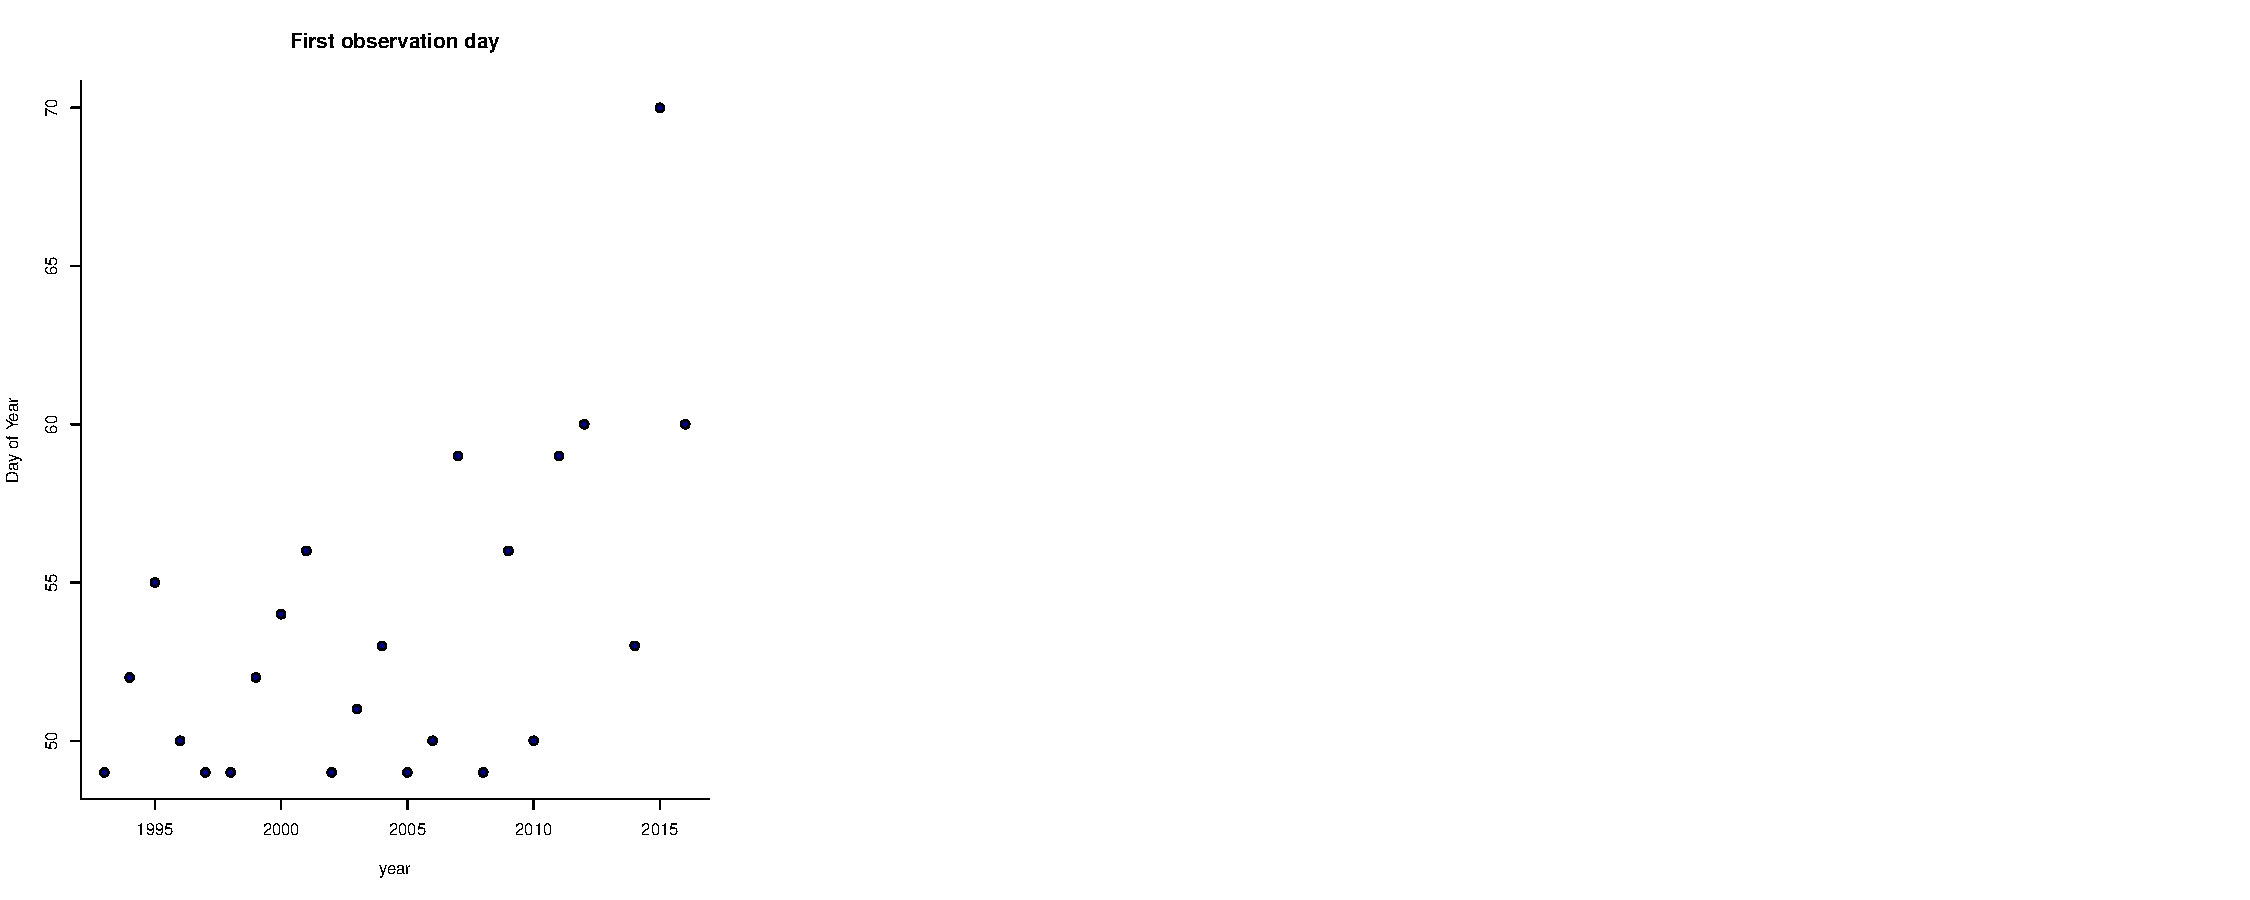
\includegraphics[width=0.8\textwidth]{../analyses/orcaphen/figures/limekilntrends_dat.pdf} 
\caption{\textbf{SRKW phenology at Lime Kiln State Park is shifting}, which the day of year of first sighting getting later (A) and the day of year of last sighting getting earlier frmo 1994-2017. These trends are associated with a decrease in the amount of time SRKWs are spending near Lime Kiln: the number of days on which SRKWs were observed ("whale days") is has declined since 1994. }
\label{fig:limetime}
\end{figure}

\begin{figure}[p]
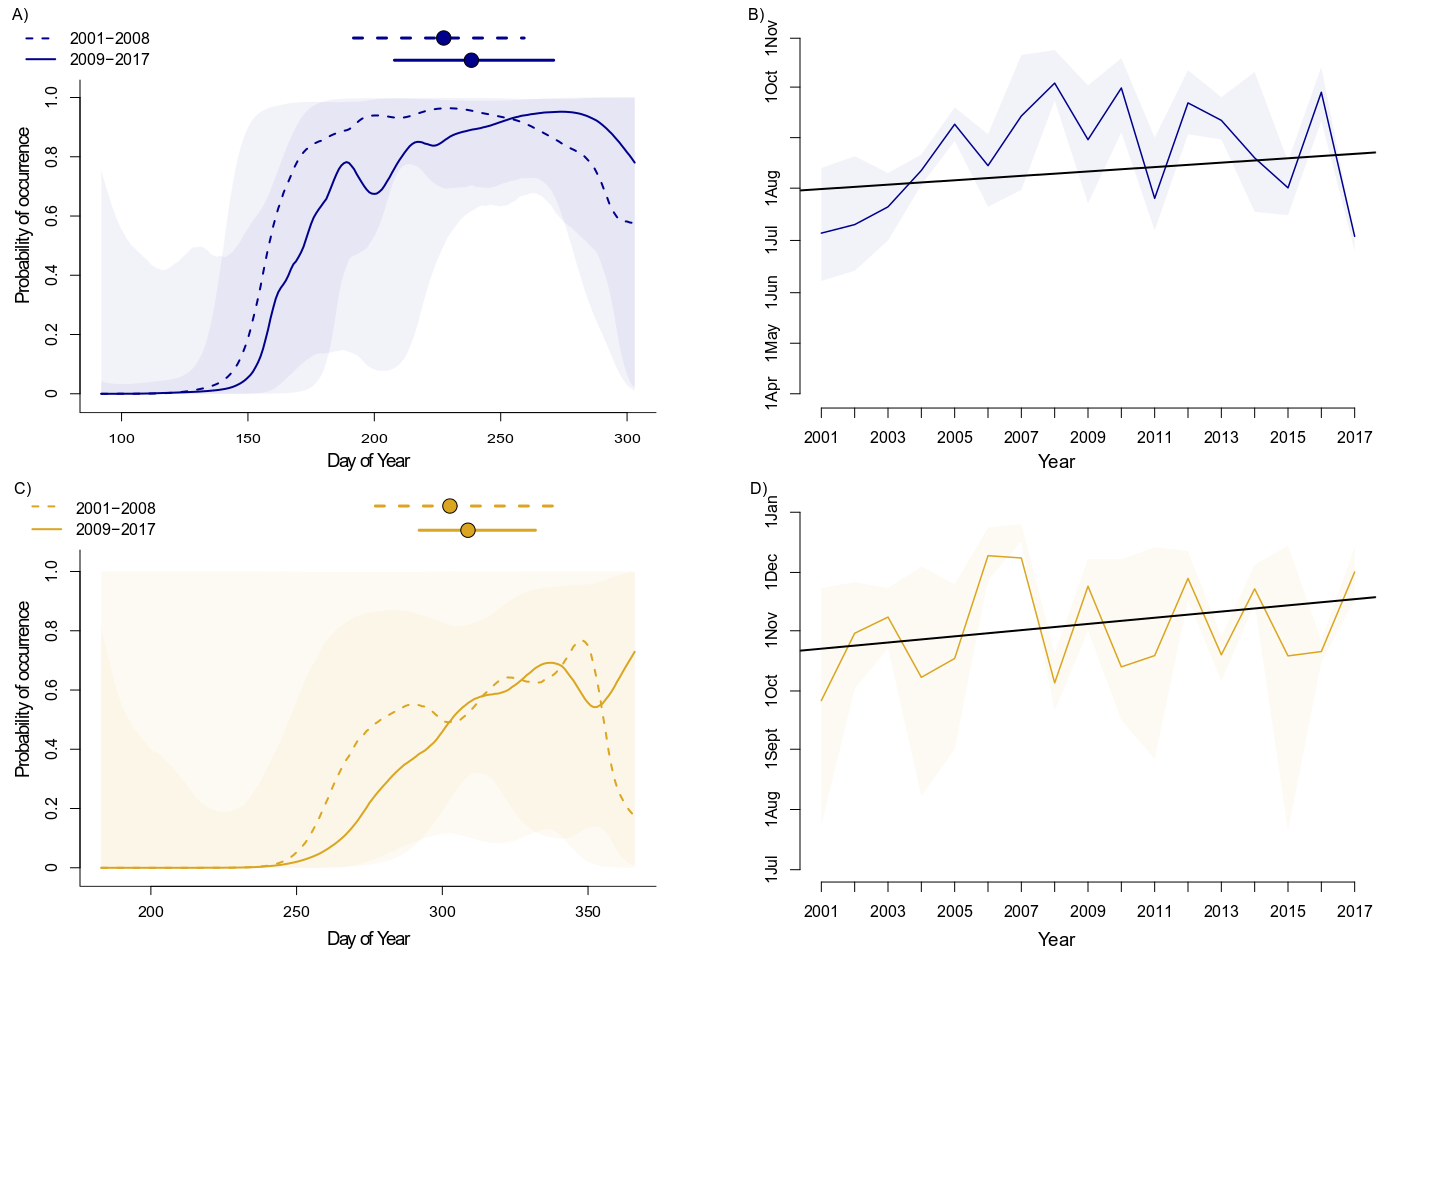
\includegraphics[width=0.8\textwidth]{../analyses/figures/proboccK_4panels.png} 
\caption{\textbf{K-pod activity varies seasonally in the Central Salish Sea (A) and Puget Sound proper (C).} This phenology has shifted later in recent years in the Central Salish Sea (B) and in Puget Sound (D). The shift toward later arrival in the central Salish Sea is evident the estimated probabilities of occurrence from the occupancy models for K-pod (A,C) as well as the linear trends in peak occurrence probability from 2001-2017 (B,D). Shading around lines represents 50\% credible intervals (95\% credible intervals in Table SX). 
}
\label{fig:Kprobs}
\end{figure}


\begin{figure}[p]
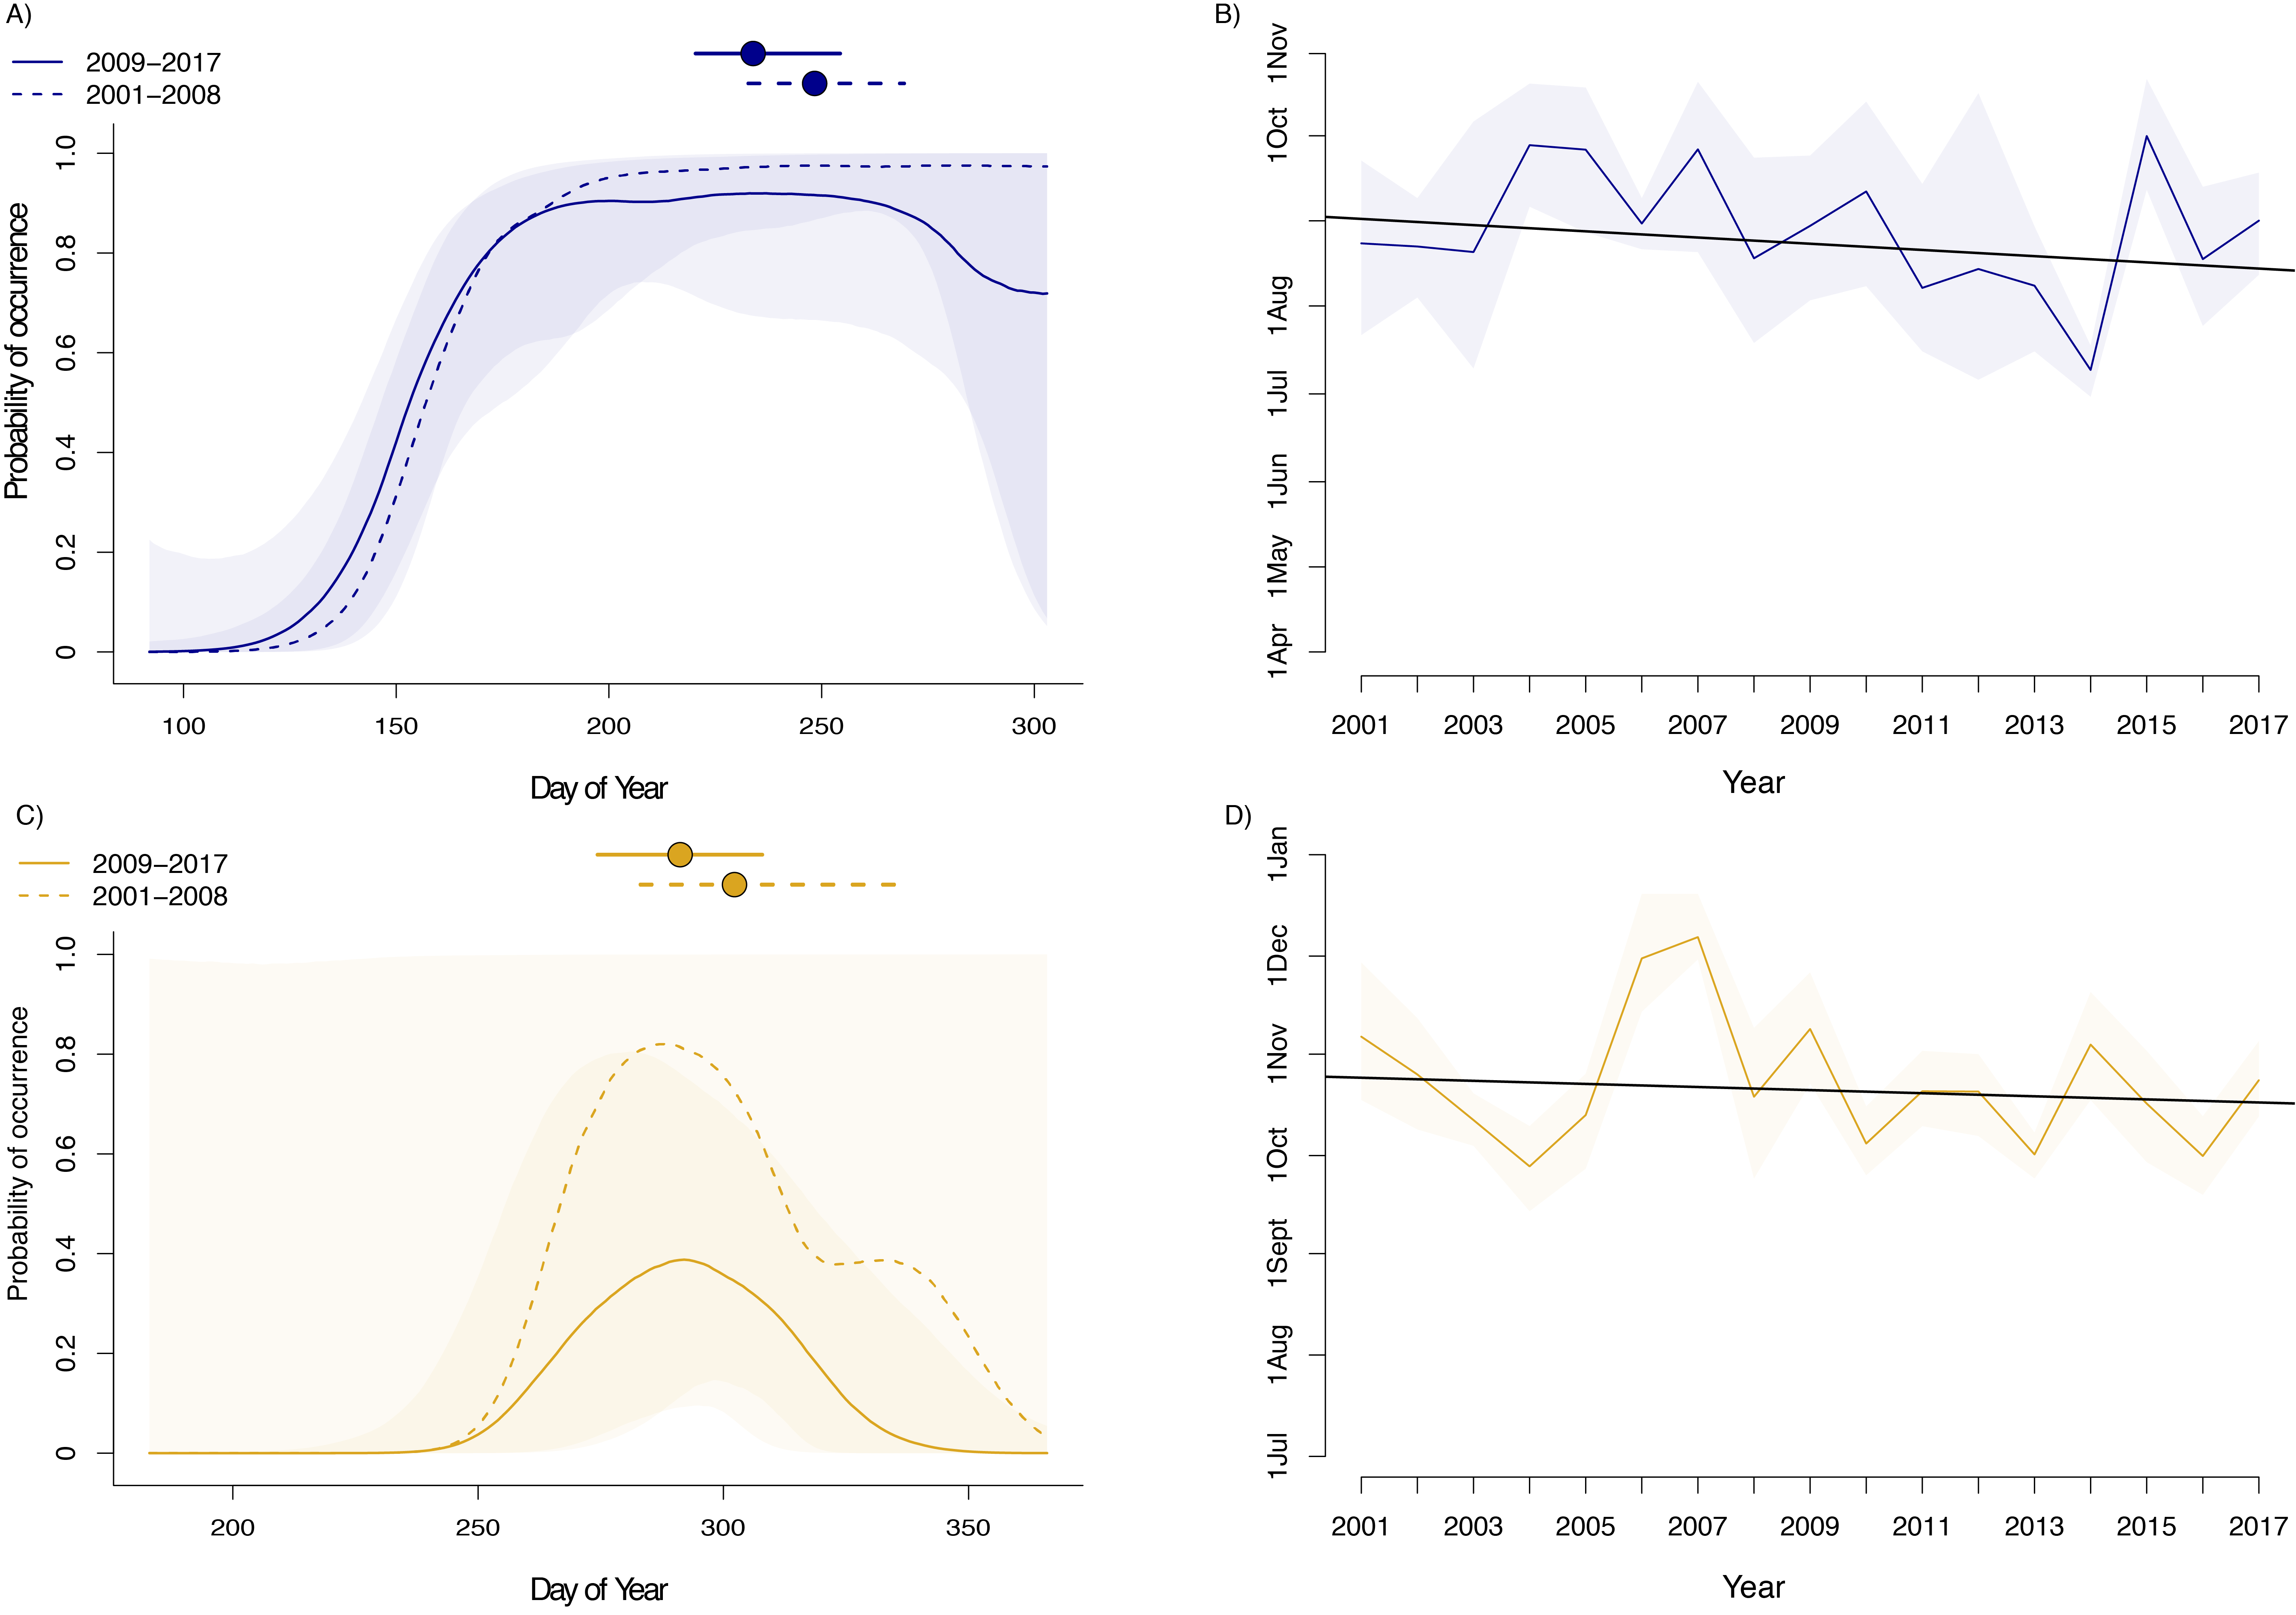
\includegraphics[width=0.8\textwidth]{../analyses/figures/proboccL_4panels.png} 
\caption{\textbf{L-pod activity varies seasonally in the Central Salish Sea (A) and Puget Sound proper (C)}. This phenology has shifted later in recent years in the Central Salish Sea (B) and in Puget Sound (D). The shift toward later arrival in the central Salish Sea is evident the estimated probabilities of occurrence from the occupancy models for K-pod (A,C) as well as the linear trends in peak occurrence probability from 2001-2017 (B,D). Shading around lines represents 50\% credible intervals (95\% credible intervals in Table SX). 
}
\label{fig:Lprobs}
\end{figure}

%%%%%%%%%%%%%%%%%%%%%%%%%%%%%%%%%%%%%%
  \end{document}
%%%%%%%%%%%%%%%%%%%%%%%%%%%%%%%%%%%%%%
